\subsection{introduction}

\begin{frame}{Audio signal processing and sound propagation}

    \begin{columns}[T,onlytextwidth]

        \begin{column}{.48\textwidth}
            \begin{block}{Sound propagation is}
                \begin{itemize}
                \item completely ignored
                \item assumed free-field case (\textit{anechoic})
                \item model it full (\textit{reverberant})
                \item \textit{learned} it full (\textit{reverberant})
                \item model few early echoes (\textit{multipath})
            \end{itemize}
            All methods can be grouped accordingly
            \end{block}
        \end{column}

        \begin{column}{.48\textwidth}
            \centering
            \only<1>{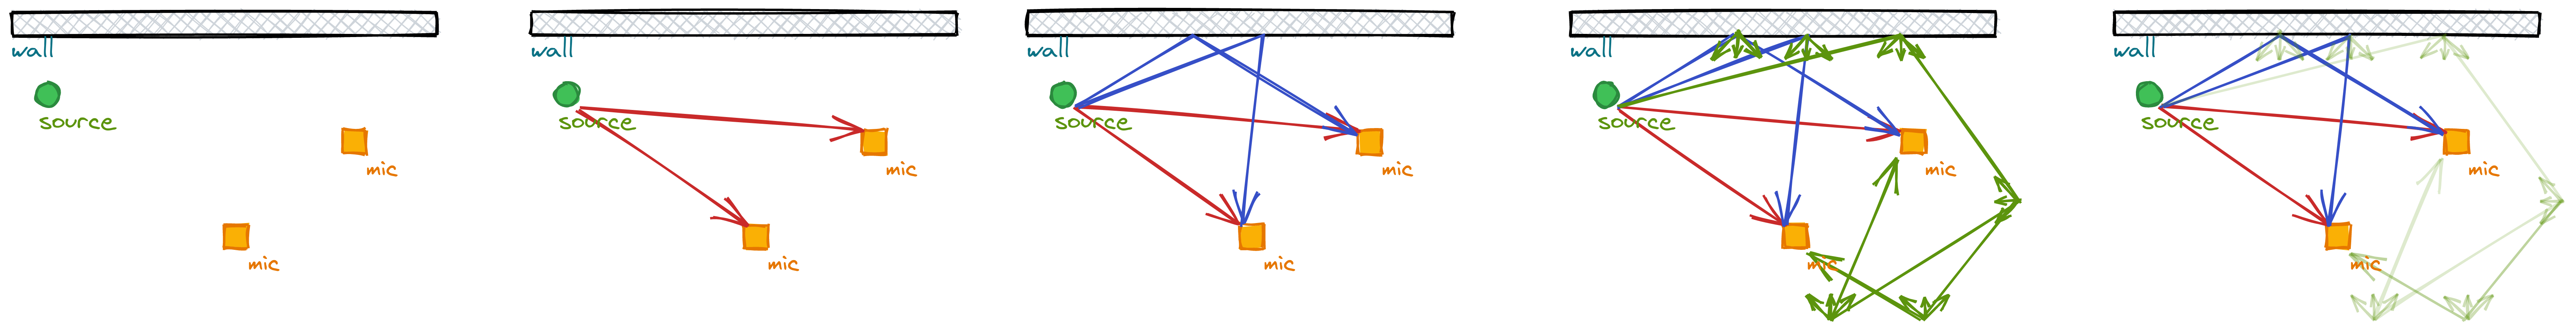
\includegraphics[trim={0 0 680em 0},clip,width=.8\textwidth]{figures/prop_it.png}}
            \only<2>{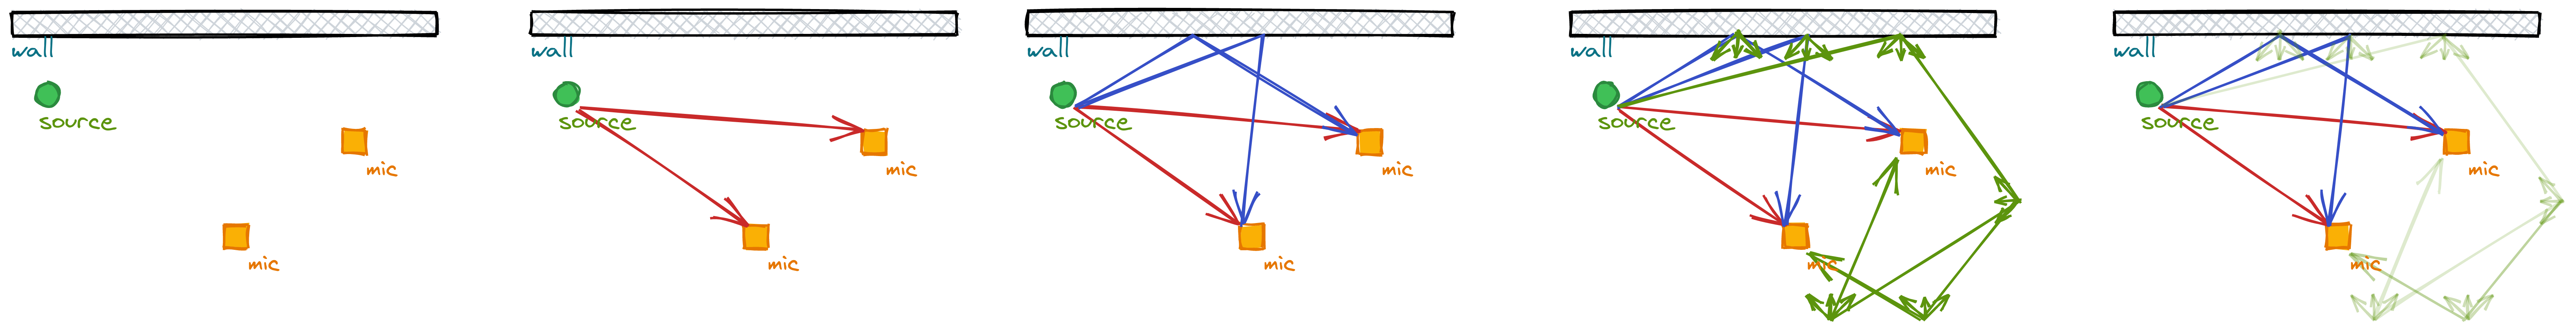
\includegraphics[trim={670em 0 5em 0},clip,width=.8\textwidth]{figures/prop_it.png}}

            \vspace{-2.3em}
            \begin{equation*}
                \begin{aligned}
                    x_i(t) &= (h_i \ast s)(t)\\
                    h_i( t) &= \textcolor{myred}{h_i^d(t)} + \textcolor{myblue}{h_i^e(t)} + \textcolor{mygreen}{h_i^r(t)}
                \end{aligned}
            \end{equation*}
        \end{column}

    \end{columns}

    % \begin{alertblock}{$\Leftarrow$ \textbf{strong early reflection} and \textbf{strong reverberation} level}
    %     \begin{itemize}
    %         \item detrimentally affect typical Audio Scene Analysis algorithm
    %         \item undesired interfering source
    %         \item undesired position of the true sources (TDOA disambiguation)
    %     \end{itemize}

    % \end{alertblock}
    \begin{block}{Recall}
        \begin{itemize}
            \item anechoic case $\implies$ simple mapping, but incoherence processing
            \item reverberant case $\implies$ hard mapping and estimation, but coherent processing
        \end{itemize}
        \hfill \textcolor{myred}{\textbf{What can we do with echoes?}}
    \end{block}
\end{frame}

\begin{frame}{Echo-aware Application}

    \begin{block}{Echoes = same content, different time/direction}
        \centering
        \only<1>{\adjincludegraphics[Clip={0\width} {0\height} {.66\width} {0\height},width=0.6\textwidth]{figures/echo_aware.png}}
        \only<2>{\adjincludegraphics[Clip={.33\width} {0\height} {.33\width} {0\height},width=0.6\textwidth]{figures/echo_aware.png}}
        \only<3>{\adjincludegraphics[Clip={.66\width} {0\height} {.00\width} {0\height},width=0.6\textwidth]{figures/echo_aware.png}}
    \end{block}


    Recent literature on echo-aware processing:
    \begin{columns}[T,onlytextwidth]
        \column{.32\textwidth}
        \begin{block}{\textbf{What?}}
            \small
            Echoes = repetitions
            \begin{itemize}
                \item Sound Source Separation
                \item Speech Enhancement
                \\\textcolor{gray}{\footnotesize(Dereverberation, Denoising, Room Equalization)}
            \end{itemize}
        \end{block}

        \column{.32\textwidth}
        \begin{block}{\textbf{Where?}}
            \small
            Echoes $\in$ indoor propagation
            \begin{itemize}
                \item Sound Source Localization
                \item Microphone Calibration
                \item Room Geometry Reconstruction
            \end{itemize}
        \end{block}

        \column{.32\textwidth}
        \begin{block}{\textbf{How?}}
            \small
            Echoes $\in$ sound propagation
            \begin{itemize}
                \item Blind Channel Estimation
                \item Acoustic Measurements
            \end{itemize}
        \end{block}
    \end{columns}

    \begin{center}
        \textcolor{gray}{\small (In-depth literature review in the manuscript.)}
    \end{center}
\end{frame}

\subsection{mirage}

\begin{frame}{\mirage - Sound Source Locatization with Echoes}

    \vspace*{5mm}
    \begin{columns}

        \begin{column}{0.5\textwidth}
            \begin{block}{The \alert{Picnic} Scenario:}
                \begin{itemize}
                    \small
                    \item One source
                    \item Two microphones
                    \begin{itemize}
                        \item[$\rightarrow$] passive scenario
                        \item[$\rightarrow$] generalizable to more pairs
                    \end{itemize}
                    \item Close to a very reflective surface
                    \begin{itemize}
                        \item[$\rightarrow$] First echo = Strongest echo
                        \item[$\rightarrow$] $\alpha_\text{picnic}$ const. $\forall f$
                        \item[$\rightarrow$] table-top device
                    \end{itemize}
                \end{itemize}
            \end{block}
        \end{column}

        \begin{column}{0.5\textwidth}
            \centering
            \only<1>{\adjincludegraphics[Clip={0\width} {0\height} {.5\width} {0\height},width=0.9\textwidth]{figures/mirage.png}}
            \only<2>{\adjincludegraphics[Clip={0.5\width} {0\height} {0\width} {0\height},width=0.9\textwidth]{figures/mirage.png}}
        \end{column}
    \end{columns}

    \vfill

    \begin{columns}[T,onlytextwidth]

        \begin{column}{0.5\textwidth}
            \begin{block}{How to access the \textit{image} microphones?}
                \\$\implies$ each pair is augmented with echoes
            \end{block}
            \begin{center}
                \textcolor{myred}{\textbf{Mirage Array}}
            \end{center}
            \textbf{idea:} use SSL algorithm on it
            \\\textbf{recall:} echoes are known
        \end{column}

        \begin{column}{0.5\textwidth}
            \centering
            \includegraphics<2>[width=\textwidth]{figures/rirs1.pdf}
            \includegraphics<3>[width=\textwidth]{figures/rirs2.pdf}
            \includegraphics<4>[width=\textwidth]{figures/rirs3.pdf}
            \includegraphics<5>[width=\textwidth]{figures/rirs4.pdf}
        \end{column}
    \end{columns}


\end{frame}

\begin{frame}{\mirage - Sound Source Locatization with Echoes}

    \begin{columns}[T,onlytextwidth]
        \column{0.6\textwidth}
        \begin{block}{SSL with 2 microphones}
            \begin{itemize}
                \item 1D SSL: only angle of arrival (AOA)
                \item e.g. GCC-PHAT for TDOA estimation~\cite{knapp1976generalized}
                \\\textcolor{gray}{\small (known limitation, but good in practice)}
            \end{itemize}
        \end{block}
        \column{0.38\textwidth}
        \adjincludegraphics[Clip={0\width} {0.5\height} {0\width} {0\height},width=0.8\textwidth]{figures/ssl.png}
    \end{columns}

    \begin{columns}[T,onlytextwidth]
        \column{0.6\textwidth}
        \begin{block}{SSL with more microphones}
            \begin{itemize}
                \item 2D SSL: azimuth and elevation
                \item For each pair $p$:
                \\\hspace{1em} AOA$_p \gets$ TDOA-based 2-mic-SSL
                \item ``Fuse''  together all the observation
                \\(Angular spectra, Probability distributions)
                \item e.g. SRP-PHAT~\cite{dibiase2001robust}
            \end{itemize}
        \end{block}
        \column{0.38\textwidth}
        \adjincludegraphics[Clip={0\width} {0\height} {0\width} {0.5\height},width=0.9\textwidth]{figures/ssl.png}
    \end{columns}

    \textbf{Baseline:} GCC-PHAT on true microphones

    \textbf{Proposed Approach:} using \lantern (DNN-based TDOA estimation)
    \begin{description}
        \item[issue:] just punctual estimation cannot be ``fused''
        \item[solution:] use \lantern in generative mode (mic pos assumed known)
    \end{description}
\end{frame}

\begin{frame}{\mirage - Results}

    \textbf{Data:} virtually generated closeddataset as for \lantern
    \\\textbf{Metric:} angular mean error and accuracy (thr=10, 20)

    \begin{columns}[T,onlytextwidth]

        \begin{column}{.4\textwidth}
        \begin{block}{AOA estimation}
            \begin{itemize}
                \item[\cmark] Similar when wn
                \item[\xmark] Huge drop when noise
                \item[\xmark] Huge drop when speech and noise
            \end{itemize}
        \end{block}
        \end{column}

        \begin{column}{.58\textwidth}

            \centering
            \small
            \begin{tabular}{cl|cc}
            \toprule
            \mathtt{AOA} &             &    \multicolumn{2}{c}{ACCURACY}  \\
                       & Input         &  $\theta<\ang{10}$ &  $\theta<\ang{20}$ \\
            \midrule
            MIRAGE     &   wn          &    4.10 (77)    &  5.97 (97)  \\
            MIRAGE     &   wn+n        &    5.00 (26)    &  9.89 (54)  \\
            GCC-PHAT   &   wn          &    4.22 (81)    &   6.19 (97) \\
            GCC-PHAT   &   wn+n        &    4.03 (65)    &   5.34 (83) \\
            \visible<2->{MIRAGE     &   sp          &    4.83 (63)    &  7.26 (82)  }\\
            \visible<2->{MIRAGE     &   sp+n        &    4.60 (16)    &  9.88 (35)  }\\
            \visible<2->{GCC-PHAT   &   sp 		   &    4.08 (82)    &   5.34 (97)  }\\
            \visible<2->{GCC-PHAT   &   sp+n        &    4.70 (19)    &   8.38 (32) }\\
            \bottomrule
        \end{tabular}
        % \begin{column}{.74\textwidth}

        %     \centering
        %     \small
        %     \begin{tabular}{cl|ccc|cc}
        %     \toprule
        %     &                  &         & nRMSE                         &              &\multicolumn{2}{c}{ACCURACY}  \\
        %     & Input            &    \scriptsize{TDOA}    &   \scriptsize{iTDOA} 		 &     \scriptsize{TDOE} 		 & $\theta<\ang{10}$ &  $\theta<\ang{20}$ \\
        %     \midrule
        %     MIRAGE     &   wn          &    0.18 & 0.28          &    0.25 	         & 4.10 (77)    &  5.97 (97) \\
        %     MIRAGE     &   wn+n        &    0.68 & 0.69          &    0.89 			 & 5.00 (26)    &  9.89 (54) \\
        %     MIRAGE     &   sp          &    0.31 & 0.34          &    0.56           & 4.83 (63)    &  7.26 (82) \\
        %     MIRAGE     &   sp+n        &    0.99 & 0.98   	     &    1.48 			 & 4.60 (16)    &  9.88 (35) \\
        %     GCC-PHAT   &   wn          &    0.21 &     -  		 &       -			 & 4.22 (81)    &   6.19 (97) \\
        %     GCC-PHAT   &   wn+n        &    0.68 &     -  		 &       -			 & 4.03 (65)    &   5.34 (83) \\
        %     GCC-PHAT   &   sp 		   &    0.32 &     -  		 &       -			 & 4.08 (82)    &   5.34 (97) \\
        %     GCC-PHAT   &   sp+n        &    1.38 &     -  		 &       -			 & 4.70 (19)    &   8.38 (32) \\
        %     \bottomrule
        % \end{tabular}
        \end{column}
    \end{columns}

    \vspace{5mm}
    \begin{columns}[T,onlytextwidth]
        \begin{column}{.25\textwidth}
            \begin{block}{2D SSL estimation}
                \textcolor{gray}{\small (both Az. and El.)}
            \end{block}
        \end{column}

        \begin{column}{.74\textwidth}
            \centering
            \small
            \begin{tabular}{cl|cc|cc}
            \toprule
            \textbf{DoA}      &               &  \multicolumn{2}{c|}{ACCURACY} &   \multicolumn{2}{c}{ACCURACY} \\
                            &               &  \multicolumn{2}{c|}{$<\ang{10}$} &   \multicolumn{2}{c}{$<\ang{20}$} \\
                            &    Input    &  $\theta$ &  $\phi$ &  $\theta$ &  $\phi$ \\
            \midrule
            MIRAGE &  wn           &   4.5 (59) &  3.9 (71) &   6.8 (79) &   5.9 (88) \\
            MIRAGE &  wn+n     &   4.4 (18) &  5.5 (26) &   9.4 (35) &  11.1 (66) \\
            MIRAGE &  sp       &   4.6 (45) &  4.8 (59) &   8.1 (71) &   7.2 (83) \\
            MIRAGE &  sp+n &   5.2 (17) &  5.9 (12) &  10.7 (38) &  12.3 (43) \\
            \bottomrule
        \end{tabular}

        \end{column}

    \end{columns}

    \begin{center}
        \textcolor{mygreen}{\cmark \: \parbox{12em}{Solved ``impossible''\\localization}}
        \quad \textcolor{myred}{\xmark \: \parbox{12em}{Performance depending on\\echo estimation}}
    \end{center}

\end{frame}


% \subsection{separake}

% \begin{frame}


% \end{frame}

% \subsection{Interim conclusion (3/4)}

% \begin{frame}{Interim conclusion (3/4)}
%     \begin{block}{Echo-aware Audio Scene Analysis}
%         \begin{itemize}
%             \item[\cmark] vast gamma of problems
%             \\$\hookrightarrow$ not limited to audio (e.g., seismology, medical imaging, astrophysics, etc.)
%             \item[\cmark] between anechoic and reverberant propagation
%             \item[\cmark] physical-interpretation (with virtual microphones)
%             \item[\xmark] performance depending on the quality of the echo-estimation
%             \\still very challenging task
%             \item[\xmark] ....
%         \end{itemize}
%     \end{block}

%     \vfill

%     \begin{block}{\mirage \& echo-aware SSL}
%         \begin{itemize}
%             \item[\cmark] impossible 2D localization with only 2 microphones
%         \end{itemize}
%     \end{block}

%     \vfill

%     \begin{block}{\separake \& echo-aware SSS}
%         \begin{itemize}
%             \item nice
%         \end{itemize}
%     \end{block}
% \end{frame}